\documentclass[11pt,letterpaper]{article}
\usepackage[margin=1in]{geometry}
\usepackage{setspace}
\usepackage{enumitem}
\usepackage{array}
\usepackage{booktabs}
\usepackage{tabularx}
\usepackage{graphicx}
\usepackage{titlesec}
\usepackage{fancyhdr}
\usepackage[T1]{fontenc}
\usepackage[utf8]{inputenc}
\usepackage{lmodern}

\setstretch{1.03}
\pagestyle{empty}
\setlength{\parindent}{15pt}
\setlength{\parskip}{4pt}
\setlist{nosep,leftmargin=0.24in}
\titlespacing*{\section}{0pt}{0.35em}{0.1em}
\titlespacing*{\subsection}{0pt}{0.25em}{0.08em}
\titleformat{\section}{\normalfont\bfseries\large}{}{0pt}{}
\titleformat{\subsection}{\normalfont\bfseries}{}{0pt}{}

\begin{document}
\begin{center}
{\Large\bfseries Project Description}\\[0.05in]
{\normalsize Mostafa Rezaali}\\
{\normalsize NSF AGS-PRF Application}
\end{center}
\vspace{-0.08in}
\section*{Project Title}
\textbf{Postdoctoral Fellowship: AGS-PRF: Probabilistic Prediction of Heat Waves and Flash Droughts Using Physics-Informed Conditional Flow Matching on an Icosahedral Mesh}

\section*{Motivation and Central Hypothesis}
Heat waves and flash droughts are compound hydroclimate hazards with large consequences for public health, energy demand, water resources, ecosystems, and agriculture. Their impacts often emerge on decision horizons of two to four weeks, when emergency managers, utilities, farmers, and public-health agencies still have time to act, but when deterministic forecast skill is often weak. Predictability at these leads is not purely local. It reflects slowly evolving ocean-atmosphere patterns, stationary waves, soil-moisture memory, radiative seasonality, synoptic persistence, and land-surface feedbacks. My central hypothesis is that a graph-based conditional flow model, trained directly on high-resolution U.S. temperature anomalies while conditioned on global circulation and teleconnection states, can reveal and exploit a measurable but spatially heterogeneous week-3 signal for extreme heat and flash-drought precursors.

\section*{Preliminary Work and Model Foundation}
I have implemented MeshFlowNet, a GraphCast-style icosahedral mesh encoder-processor-decoder for direct 15-day CONUS daily maximum temperature prediction. The model uses current and lagged local PRISM temperature anomalies, atmospheric and land-surface fields, topography, latitude, longitude, seasonal insolation, land mask, five teleconnection indices, and a 59-channel global ERA5/coarse atmospheric context stack. It supports deterministic residual prediction and probabilistic conditional-flow-matching modes. The current deterministic five-fold leave-years-out hindcast covers MJJAS 1981--2023, with each year predicted by a model that did not train on that year. Across 5,332 samples, stitched model temporal anomaly correlation is 0.1016 compared with 0.0735 for persistence, a +0.0281 improvement.

\begin{center}
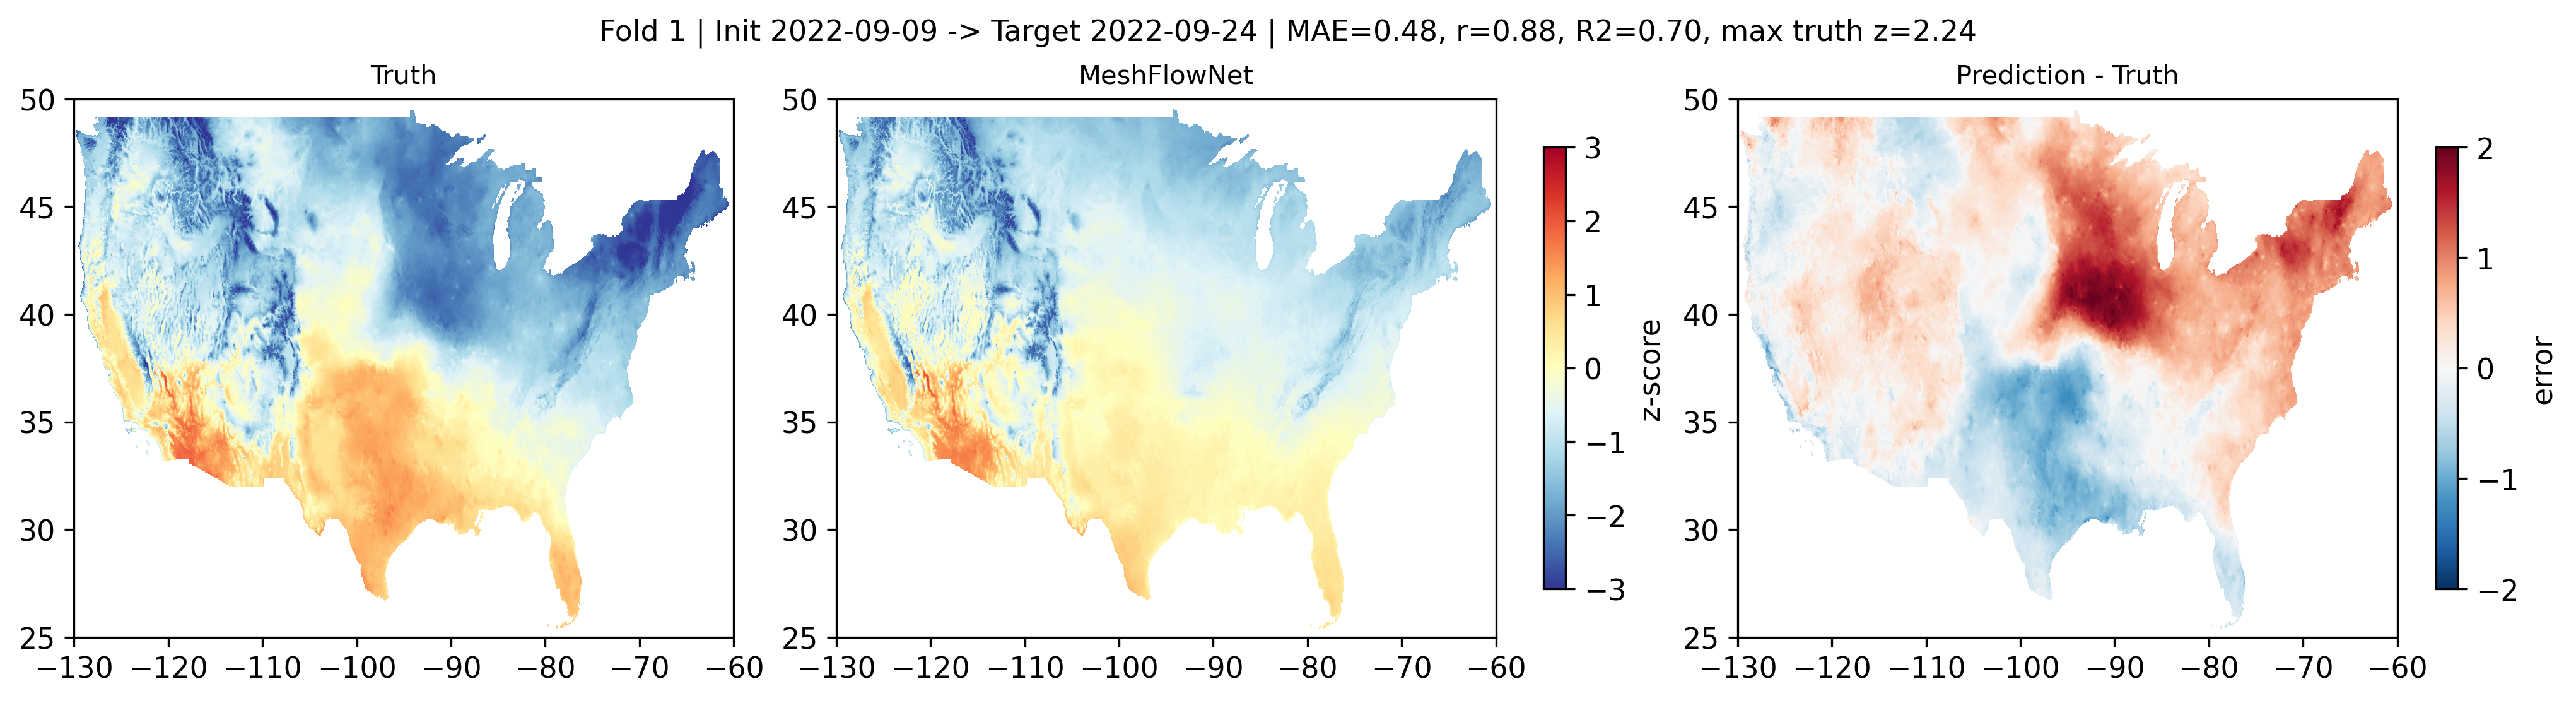
\includegraphics[width=0.96\textwidth]{figures/figure_preliminary_prediction.png}\\[-0.04in]
\footnotesize\textbf{Figure 1.} Example 15-day hindcast from the preliminary MeshFlowNet system, showing verifying anomaly, direct model prediction, and prediction-minus-truth error over CONUS.
\end{center}

These preliminary results are not presented as an operational system. They show that the model extracts nontrivial anomaly signal at a difficult lead time and justify a systematic postdoctoral investigation of predictability, uncertainty, and physical interpretation. The fellowship will convert this foundation into a calibrated probabilistic framework and a documented scientific benchmark for week-3 heat and flash-drought-relevant risk.

\section*{Aim 1: Build a Calibrated Conditional-Flow Forecast System}
The first aim will convert the current deterministic residual model into a probabilistic forecast system. The deterministic branch predicts $y(t+15)$ as persistence plus a learned residual in one forward pass. The conditional-flow branch will learn a velocity field from initialization-time state to the verifying anomaly field, conditioned on teleconnection indices and global atmosphere/ocean fields. Ensembles will be generated by sampling the flow and by training multiple seeds per cross-validation fold. Calibration will be assessed with continuous ranked probability score, reliability diagrams for exceedance of local 90th and 95th percentiles, rank histograms, Brier score, and spatially stratified spread-skill relationships.

This aim will test whether conditional flow matching can deliver useful uncertainty rather than only sharper deterministic maps. A successful result will be a reproducible probabilistic benchmark for week-3 U.S. heat prediction. If the CFM ensembles are underdispersed, I will test temperature scaling, ensemble perturbations, and loss weighting for extreme cases. If the ensembles are sharp but poorly calibrated, I will diagnose whether the problem is regional, seasonal, or associated with specific circulation regimes.

\section*{Aim 2: Diagnose Sources of Subseasonal Predictability}
The second aim will use controlled ablations and interpretable diagnostics to determine which features carry week-3 skill. I will compare models trained with: local persistence only; local meteorology plus static and seasonal terms; teleconnection indices; global ERA5 fields; and the full conditioning stack. The analysis will produce per-pixel temporal anomaly correlation, skill over persistence, regional summaries for NOAA climate regions, block-bootstrap significance tests by year, and event composites for strong teleconnection regimes.

The scientific target is not only a higher metric, but a physical account of where AI forecast skill is consistent with known pathways such as Pacific-North American wave trains, moisture transport, soil-moisture feedback, subtropical ridge variability, and persistent high-pressure anomalies. These diagnostics will help distinguish robust predictive signal from overfitting or spatially smooth climatological reconstruction.

\section*{Aim 3: Connect Heat Prediction to Flash-Drought-Relevant Risk}
The third aim will connect temperature-anomaly prediction to flash-drought precursors by evaluating rapid intensification of heat and atmospheric demand in conjunction with antecedent soil-moisture state. The model already ingests soil moisture, humidity, winds, sea-level pressure, radiation, and large-scale circulation fields. I will evaluate whether the learned representations anticipate co-occurring hot, dry, high-demand regimes over agriculturally important regions. Products will be reported as calibrated probabilistic exceedance maps, regional time series, and case studies rather than deterministic binary declarations.

\section*{Data and Model Architecture}
The hindcast system will use PRISM daily maximum temperature over CONUS at 0.04-degree resolution, ERA5 atmospheric variables and global context fields, teleconnection indices, topography, latitude, longitude, land mask, top-of-atmosphere insolation, and seasonal encodings. The current local input stack contains current and lagged PRISM temperature fields; geopotential, soil moisture, sea-level pressure, 2-m temperature, 850-hPa humidity, 850-hPa temperature and winds, 300-hPa geopotential; topography; latitude and longitude; day-of-year sine and cosine; insolation; and land mask. The global context stack contains SST, OLR, winds, geopotential, temperature, humidity, surface pressure, sea-level pressure, and total column water vapor across multiple levels.

\begin{center}
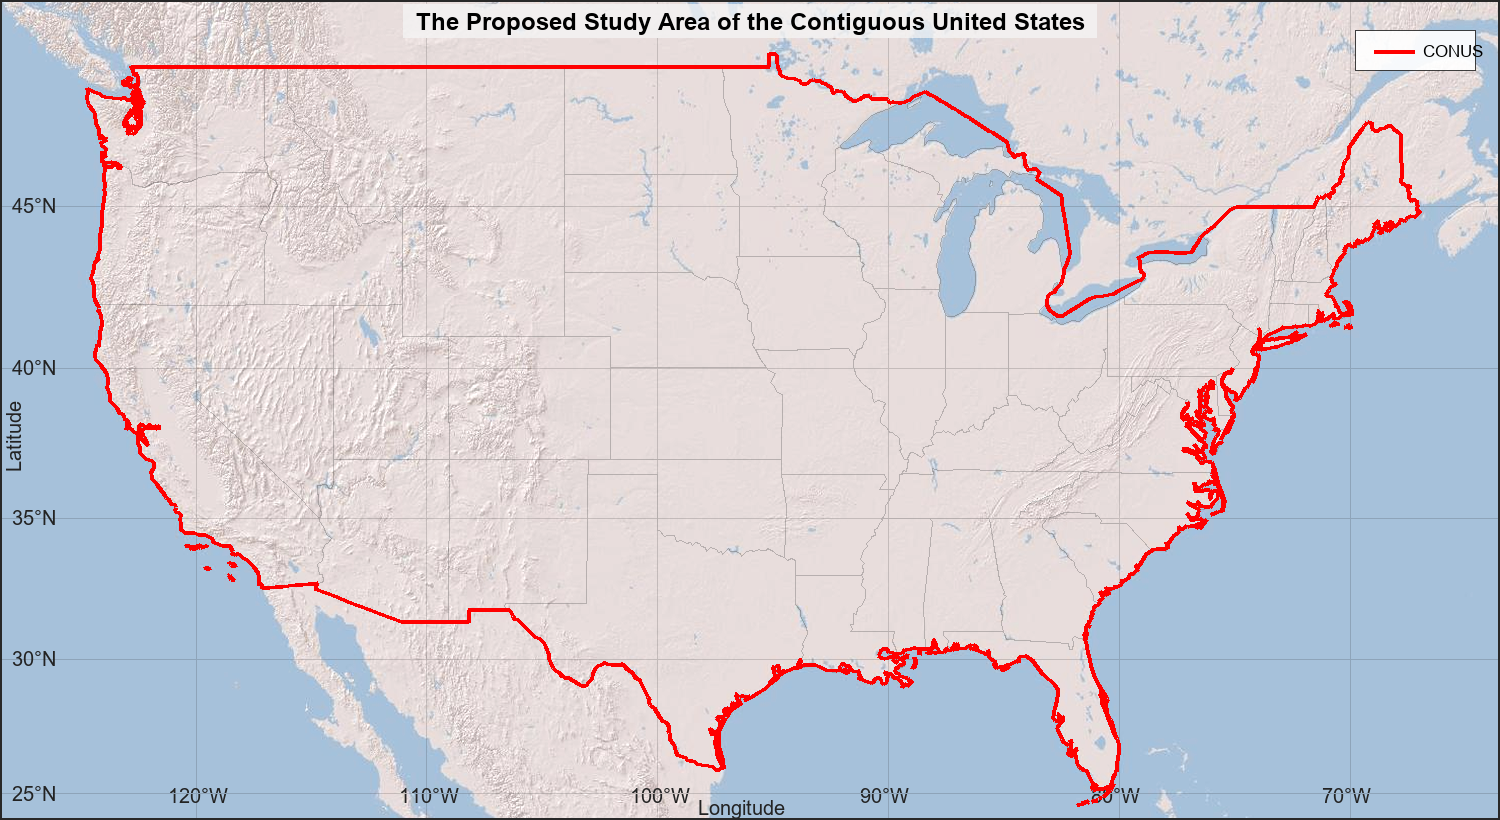
\includegraphics[width=0.86\textwidth]{figures/figure_study_area_conus.png}\\[-0.04in]
\footnotesize\textbf{Figure 2.} Proposed study domain over the contiguous United States for model training, validation, regional diagnostics, and heat-risk evaluation.
\end{center}

MeshFlowNet maps the CONUS grid to an icosahedral mesh, performs message passing with graph interaction networks and conditioning, and decodes back to the land grid. This representation preserves global-to-regional context while avoiding purely convolutional locality. The probabilistic branch will use continuous-time embeddings and conditional flow matching; the deterministic branch will remain as a transparent baseline and an efficient ablation.

\section*{Evaluation and Validation}
All claims will be based on leave-years-out cross-validation over 1981--2023. Metrics will include temporal anomaly correlation, spatial anomaly $R^2$, MAE, MSE skill relative to persistence, CRPS, reliability of extreme exceedance probabilities, and block-bootstrap confidence intervals. Baselines will include climatology, persistence, ridge regression on teleconnection/global summary features, and published operational S2S reference skill where metric and domain are comparable. I will report negative or regionally limited results explicitly because understanding where AI models fail is essential for trustworthy climate-risk use.

\section*{Detailed Research Activity Plan}
Months 1--3 will focus on data audit, cross-validation lock-in, and reproducible baseline runs. Months 4--6 will finalize deterministic baselines and regional skill maps. Months 7--12 will train probabilistic CFM ensembles and complete CRPS, reliability, and spread-skill evaluation. Months 13--16 will complete ablations and teleconnection-regime diagnostics. Months 17--20 will connect heat prediction to flash-drought-relevant risk products. Months 21--24 will finalize manuscript submissions, public documentation, derived product release, and conference dissemination.

\section*{Justification for Host Institution and Sponsoring Scientist}
The proposed host institution is University of Florida, Department of Geography. The host setting is scientifically appropriate because it provides deep expertise in climatology, climate extremes, hydroclimatology, geospatial analysis, and environmental prediction. The proposed sponsoring scientist is David Keellings, University of Florida, whose expertise in heat waves, climate extremes, and applied climatology directly aligns with the proposed work. This environment will provide disciplinary grounding for interpreting AI forecast skill, evaluating physical consistency, and translating probabilistic predictions into climate-risk knowledge.

The fellowship will support a transition from doctoral model development to an independent research program in probabilistic subseasonal predictability, uncertainty quantification, and open forecast diagnostics. The sponsoring scientist will support regular research meetings, manuscript planning, proposal-development feedback, conference preparation, mentoring opportunities, and career-development milestones.

\section*{Facilities and Resources}
The project will use research computing resources, Python/PyTorch software environments, geospatial and climate-data analysis tools, and publicly available PRISM/ERA5-derived data workflows. The local codebase already runs on GPU-equipped computing systems and includes scripts for training, hindcast export, bootstrap statistics, baseline comparison, temporal anomaly correlation maps, sample maps, and CRPS/reliability analysis. These resources are sufficient for the proposed two-year work plan.

\section*{Intellectual Merit}
The intellectual merit is the integration of subseasonal predictability theory, graph neural weather models, and probabilistic flow matching. The project will advance knowledge by quantifying when global and land-surface information improves 15-day U.S. heat prediction beyond persistence; producing spatially explicit diagnostics of learned teleconnection skill; and testing whether conditional-flow models can provide calibrated uncertainty for regional extreme-temperature risk. The outcome will be a physically evaluated AI framework rather than a black-box score table.

\section*{Broader Impacts}
The broader impacts center on usable, transparent climate-risk intelligence and training. First, the project will produce reproducible code, derived hindcast diagnostics, and documentation suitable for students and practitioners who need to understand AI forecast limitations. Second, I will develop a short teaching module on graph neural weather prediction and uncertainty for graduate climate modeling or environmental data-science courses. Third, I will mentor undergraduate and REU students in open climate-data workflows, with attention to students entering atmospheric science from geography, environmental engineering, and data science. Fourth, the forecast diagnostics will be framed around heat-health, water, energy, and agriculture use cases where calibrated uncertainty can be more valuable than a single deterministic forecast.

\section*{Expected Products and Success Criteria}
Success will be assessed by scientific and broader-impact outputs: a documented cross-validated hindcast benchmark with uncertainty metrics; at least two manuscripts, one on model and predictability and one on physical-regime interpretation or flash-drought-relevant risk; public release of code, metadata, and nonrestricted derived products; student mentoring and teaching materials; and a clear professional transition from doctoral model development to an independent research program in AI-enabled atmospheric predictability.

\newpage
\section*{Detailed Methodological Plan: Data Assembly and Quality Control}
The first technical phase will establish a locked, auditable data pipeline. PRISM daily maximum temperature fields will be transformed into anomalies using a consistent climatological baseline and land mask. ERA5 and related atmospheric fields will be regridded or sampled consistently with the model architecture, with metadata documenting variable names, pressure levels, units, time stamps, and preprocessing choices. Teleconnection indices will be standardized using training-period statistics within each cross-validation fold to avoid leakage. Static fields, seasonal encodings, and top-of-atmosphere radiation will be versioned with the model configuration.

Quality control will include checks for missing days, temporal misalignment, duplicated files, unit inconsistency, grid mismatch, and accidental use of validation-year information during training. I will produce summary tables for sample counts by year and fold, and maps showing valid-grid coverage and climatological variance. These checks are necessary because small data-leakage or alignment errors can produce misleading gains in subseasonal AI forecasting.

\begin{center}\scriptsize
\textbf{Table 1. Core predictor groups and quality-control checks.}\\[0.03in]
\begin{tabularx}{\textwidth}{p{0.18\textwidth}p{0.34\textwidth}p{0.17\textwidth}X}
\toprule
\textbf{Group} & \textbf{Variables / fields} & \textbf{Role} & \textbf{Quality-control checks}\\
\midrule
PRISM local state & Current and lagged daily maximum temperature anomalies & Persistence memory and local anomaly structure & Missing days, land-mask consistency, anomaly baseline, no validation-year leakage\\
Atmospheric state & Geopotential, sea-level pressure, 2-m temperature, 850-hPa humidity, 850-hPa temperature/winds, 300-hPa geopotential & Synoptic and regional forcing & Unit checks, time alignment, pressure-level consistency, grid registration\\
Land-surface memory & Soil moisture, topography, land mask, latitude, longitude & Heat amplification and spatial heterogeneity & Static-field versioning, mask agreement, terrain-grid consistency\\
Seasonal forcing & Day-of-year sine/cosine, top-of-atmosphere insolation & Annual cycle and radiative context & Leap-day handling, fold-specific normalization, temporal indexing\\
Remote context & SST, OLR, winds, humidity, temperature, pressure, TCWV, teleconnection indices & Global circulation and teleconnection predictors & Training-fold standardization, field completeness, index-source audit\\
\bottomrule
\end{tabularx}
\end{center}

\newpage
\section*{Detailed Methodological Plan: Baselines and Ablations}
The second technical phase will build baselines that are scientifically interpretable. Persistence and climatology will define minimum forecast value. Ridge or regularized linear models using teleconnection and global-summary predictors will test whether nonlinear graph structure is necessary. Local-only and global-context ablations will separate skill from local memory versus remote atmospheric drivers. Static-field and seasonality ablations will test whether the model is relying on physically meaningful anomaly evolution rather than geographic memorization.

Each ablation will be evaluated with the same cross-validation years, same verification masks, and same statistical tests. Results will be summarized as regional skill tables, per-pixel maps, and event-conditioned diagnostics. This structure will make it possible to identify whether CFM improves forecast uncertainty, deterministic anomaly reconstruction, or both.

\begin{center}\scriptsize
\textbf{Table 2. Selected training and validation metrics from \texttt{cvfold2\_pub\_weekly7}.}\\[0.03in]
\begin{tabular}{rrrrrrrrr}
\toprule
\textbf{Epoch} & \textbf{Train} & \textbf{RMSE} & \textbf{R2} & \textbf{TAC} & \textbf{Wk7 TAC} & \textbf{Wk7 pers.} & \textbf{Spatial R2} & \textbf{MAE}\\
\midrule
1 & 0.398 & 0.894 & 0.183 & 0.042 & 0.112 & 0.107 & 0.208 & 0.676\\
2 & 0.283 & 0.806 & 0.337 & 0.041 & 0.111 & 0.107 & 0.330 & 0.611\\
3 & 0.234 & 0.728 & 0.459 & 0.042 & 0.103 & 0.107 & 0.444 & 0.553\\
4 & 0.223 & 0.700 & 0.499 & 0.044 & 0.094 & 0.107 & 0.494 & 0.530\\
5 & 0.218 & 0.691 & 0.513 & 0.044 & 0.087 & 0.107 & 0.513 & 0.521\\
6 & 0.219 & 0.684 & 0.522 & 0.046 & 0.084 & 0.107 & 0.523 & 0.515\\
7 & 0.207 & 0.678 & 0.531 & 0.052 & 0.089 & 0.107 & 0.531 & 0.511\\
8 & 0.207 & 0.674 & 0.536 & 0.057 & 0.091 & 0.107 & 0.535 & 0.508\\
9 & 0.207 & 0.672 & 0.539 & 0.061 & 0.094 & 0.107 & 0.537 & 0.507\\
10 & 0.182 & 0.670 & 0.541 & 0.067 & 0.102 & 0.107 & 0.539 & 0.506\\
11 & 0.189 & 0.670 & 0.541 & 0.070 & 0.103 & 0.107 & 0.539 & 0.506\\
12 & 0.198 & 0.671 & 0.540 & 0.072 & 0.103 & 0.107 & 0.537 & 0.507\\
13 & 0.186 & 0.673 & 0.538 & 0.076 & 0.106 & 0.107 & 0.535 & 0.507\\
14 & 0.180 & 0.676 & 0.533 & 0.077 & 0.106 & 0.107 & 0.531 & 0.509\\
15 & 0.168 & 0.679 & 0.529 & 0.076 & 0.107 & 0.107 & 0.528 & 0.511\\
16 & 0.177 & 0.683 & 0.523 & 0.075 & 0.103 & 0.107 & 0.522 & 0.515\\
\bottomrule
\end{tabular}\\[0.03in]
\footnotesize Values show rapid reduction in RMSE and MAE, improved validation R2, increasing full-period TAC, and weekly-7 TAC compared with the persistence reference.
\end{center}

\newpage
\section*{Detailed Methodological Plan: Conditional Flow Matching}
The CFM component will represent forecast uncertainty by learning a conditional transformation from a simple distribution to verifying temperature-anomaly fields. The conditioning variables will include current state, lagged temperature, land-surface memory, global circulation, and teleconnection state. I will evaluate multiple sampling strategies and training seeds to separate aleatoric forecast uncertainty from model-training variability.

The probabilistic output will be evaluated using distributional metrics rather than only ensemble mean performance. CRPS, reliability, spread-skill consistency, rank histograms, and exceedance-probability calibration will determine whether the forecast probabilities are useful. If the model produces visually plausible but statistically miscalibrated ensembles, calibration diagnostics will guide retraining, loss weighting, or post-processing.

\begin{center}\scriptsize
\textbf{Table 3. Model components and expected scientific contribution.}\\[0.03in]
\begin{tabularx}{\textwidth}{p{0.22\textwidth}p{0.32\textwidth}p{0.18\textwidth}X}
\toprule
\textbf{Component} & \textbf{Implementation} & \textbf{Output} & \textbf{Scientific purpose}\\
\midrule
Grid-to-mesh encoder & Maps PRISM/ERA5 fields onto an icosahedral mesh & Latent graph state & Allows regional predictions to ingest nonlocal atmospheric context\\
Graph processor & Repeated message passing with conditioning & Updated latent dynamics & Tests whether teleconnection information improves week-3 heat skill\\
Mesh-to-grid decoder & Converts graph state back to CONUS grid & 15-day anomaly field & Produces spatially explicit heat-risk diagnostics\\
Residual head & Persistence plus learned correction & Deterministic benchmark & Separates learned anomaly evolution from simple persistence\\
CFM head & Conditional velocity field and ensemble sampling & Predictive distribution & Evaluates calibrated uncertainty and exceedance probabilities\\
\bottomrule
\end{tabularx}
\end{center}

\begin{center}\scriptsize
\textbf{Table 4. Verification metrics and interpretation.}\\[0.03in]
\begin{tabularx}{\textwidth}{p{0.22\textwidth}p{0.18\textwidth}X}
\toprule
\textbf{Metric} & \textbf{Target} & \textbf{Interpretation}\\
\midrule
Temporal anomaly correlation & Deterministic skill & Tracks daily anomaly evolution at each location\\
Spatial anomaly R2 & Map fidelity & Measures predicted spatial pattern agreement\\
CRPS & Probabilistic skill & Scores full predictive distributions\\
Reliability / rank histograms & Calibration & Tests whether probabilities can be interpreted honestly\\
MSE skill vs. persistence & Practical value & Tests added value beyond a low-cost baseline\\
\bottomrule
\end{tabularx}
\end{center}

\newpage
\section*{Detailed Methodological Plan: Physical Interpretation}
A central risk in AI weather and climate prediction is that high-dimensional models can appear skillful without revealing why. To address this, the project will connect skill diagnostics to physically interpretable regimes. Composite analysis will examine years and periods with strong teleconnection signals, persistent ridging, dry soil-moisture states, and large regional heat anomalies. Regional skill will be compared across humid, arid, coastal, and continental climates, and across periods with different background circulation.

Interpretation will focus on whether skill improvements align with plausible atmospheric pathways. For example, if the model improves over persistence during certain Pacific-North American or subtropical ridge regimes, the analysis will examine whether global-context inputs are essential in those cases. If skill is limited to regions dominated by persistence, the project will state that limitation clearly.

\begin{center}\scriptsize
\textbf{Table 5. Physical interpretation matrix for regime-dependent skill.}\\[0.03in]
\begin{tabularx}{\textwidth}{p{0.20\textwidth}p{0.27\textwidth}p{0.24\textwidth}X}
\toprule
\textbf{Diagnostic} & \textbf{Comparison} & \textbf{Expected signal} & \textbf{Use in interpretation}\\
\midrule
Teleconnection composites & Strong vs. weak index states & Skill changes under remote forcing & Tests whether global context is used physically\\
Soil-moisture stratification & Dry vs. wet antecedent states & Larger heat amplification under dry soils & Links skill to land-atmosphere feedback\\
Regional grouping & West, Plains, Southeast, Northeast & Spatially heterogeneous skill & Identifies where prediction is meaningful\\
Event amplitude bins & Moderate vs. extreme anomalies & Reliability changes in tails & Tests handling of high-impact events\\
Input ablations & Full vs. local-only/global-only & Skill loss when pathways are removed & Supports interpretation of predictors\\
\bottomrule
\end{tabularx}
\end{center}

\begin{center}\scriptsize
\textbf{Table 6. Risk-management logic for model outcomes.}\\[0.03in]
\begin{tabularx}{\textwidth}{p{0.25\textwidth}p{0.32\textwidth}X}
\toprule
\textbf{Outcome} & \textbf{Response} & \textbf{Scientific value}\\
\midrule
CFM improves calibration & Release calibrated hindcast diagnostics & Demonstrates probabilistic graph-forecast utility\\
Only deterministic skill improves & Compare residual and ensemble behavior & Identifies uncertainty-modeling limitations\\
Skill is regime-limited & Publish regime-dependent predictability & Clarifies when week-3 prediction is plausible\\
Baselines match AI model & Report limits and failure modes & Prevents overclaiming and creates a benchmark\\
\bottomrule
\end{tabularx}
\end{center}

\newpage
\section*{Detailed Work Plan: Broader Impacts and Training}
The broader-impact work will be integrated with the research rather than treated as a separate activity. Reproducible code and derived diagnostics will be organized so students can follow the full workflow from data preparation to model evaluation. Teaching material will use small examples to explain graph neural weather prediction, forecast uncertainty, reliability, and the difference between experimental research products and operational guidance.

Mentoring activities will emphasize transparent evaluation, ethical use of AI, and climate-risk communication. Students will be encouraged to ask not only whether a model is accurate, but for whom, where, when, and with what uncertainty. This framing supports responsible use of AI in environmental prediction and helps broaden participation for students whose training begins in geography, environmental engineering, or data science.

\begin{center}\scriptsize
\textbf{Table 7. Two-year work plan, products, and review checkpoints.}\\[0.03in]
\begin{tabularx}{\textwidth}{p{0.13\textwidth}p{0.33\textwidth}p{0.25\textwidth}X}
\toprule
\textbf{Period} & \textbf{Research activity} & \textbf{Product} & \textbf{Checkpoint}\\
\midrule
Months 1--3 & Data audit, fold lock-in, baseline reproduction & Preprocessing and baseline report & Confirm no leakage and consistent samples\\
Months 4--6 & Deterministic model and skill maps & Regional TAC/R2 maps and tables & Identify regions with added skill\\
Months 7--12 & CFM ensembles and calibration & CRPS, reliability, rank histograms & Decide calibration strategy\\
Months 13--16 & Ablations and regime diagnostics & Teleconnection/soil-moisture composites & Link skill to mechanisms\\
Months 17--20 & Flash-drought heat-risk products & Exceedance maps and cases & Evaluate use-relevant uncertainty\\
Months 21--24 & Manuscripts, release, teaching module & Papers, repository, archive & Complete dissemination milestones\\
\bottomrule
\end{tabularx}
\end{center}

\begin{center}\scriptsize
\textbf{Table 8. Broader-impact deliverables.}\\[0.03in]
\begin{tabularx}{\textwidth}{p{0.24\textwidth}p{0.35\textwidth}X}
\toprule
\textbf{Deliverable} & \textbf{Audience} & \textbf{Planned content}\\
\midrule
Teaching module & Graduate and advanced undergraduate students & Graph weather models, uncertainty, reliability, and limitations\\
Reproducible workflow & Climate-data science learners and researchers & Data-processing scripts, model configs, diagnostics, metadata\\
Mentoring activities & REU and student researchers & Model evaluation, transparent reporting, climate-risk communication\\
Public derived products & Scientific community & Hindcast diagnostics, tables, and figure-generation workflows\\
\bottomrule
\end{tabularx}
\end{center}
\end{document}
